\documentclass{beamer}
\usepackage{graphicx}
\usepackage{wrapfig}
\usepackage{setspace}
\usepackage{xcolor}
\usetheme{Madrid}
\usecolortheme{default}

\title[21G378383]{Translation / Transliteration of Vernacular Languages from Signboards}
\subtitle{Project ID:21G378383\\Review - I}
\author[SRM Institute of Science \& Technology]{Group~Members\\RA1711003030378~Vishnu~Teja~Chikkala\\RA1711003030383~Rajpreet~Srivastav\\ \medskip{Supervised By:\\Mr.~Sunil~Kumar\\Assistant~Professor}}
\institute[]{Department of Computer Science \& Engineering\\Faculty of Engineering \& Technology\\SRM Institute of Science \& Technology}
\logo{
\includegraphics[scale=.4]{srm_logo}}
%\author{Vishnu Teja Chikkala}
\date{\today}
\begin{document}
	\begin{frame}
		\maketitle
		\date{}
			\end{frame}
	\begin{frame}[allowframebreaks]{Table of Contents} %we can expand the table of contents in more than on frame
		\tableofcontents[sections={1-6}]
	\end{frame}
	\section{Abstract}
	\begin{frame}[allowframebreaks]{Abstract}
		
	India has 22 constitutionally recognized languages written in 13 different scripts. An average traveler, when travelling to a new region, might often get confused with signboards written in an unfamiliar language. It is also impossible to have every signboard in every city / town / village written in 22 different languages, as there will not be enough room to accommodate more than 2 – 3 scripts. \par
The goal of this project is to develop an App which translates the text written on a signboard into another language as desired by the user. The user should simply point at and click a picture of the signboard using the camera of their phone and the app will translate the text written on the signboard. This will be accomplished with the use of neural networks trained for text detection, recognition and translation tasks on collected and freely-available datasets, which will be developed using Python and frameworks such as TensorFlow. The user app will be designed in Java. \par
For the scope of this project, we will design a system which works for names (such as road names, city names, shop names, organization names, etc.) which typically are not longer than 4-5 words, and support translation for 1 or 2 languages. Further scope for the project involves including support for more languages and building models to support translation / transliteration of longer pieces of text.
	\end{frame}

\section{Literature Survey}
	\begin{frame}[allowframebreaks]{Literature Survey}
	\begin{itemize}
		\item Indian community faces a “Digital Divide” due to dominance of English as mode of communication in higher education, judiciary, corporate sector and Public administration at Central level whereas the government in states work in their respective regional languages \cite{kurian2008natural} 
		\item India has 22 scheduled languages. While 99 \%  of the population speak one of these scheduled languages in various dialects (which number in the thousands) \cite{theindianexpress_2018}, according to Census 2011, the total percentage of English speakers is at 10 \%, and that too is skewed towards the urban population. \cite{s_2019} Hence, there lies a need for developing NLP architectures for facilitating flow of digital content and information in and between local, national and international levels.
		\item The above also means that a large percentage of the literate population is either monolingual or bilingual, and across 22 languages, an accessible, easy-to-use and intuitively developed system is required, which enables intercommunication.
		\item While traditionally NLP has been approached with statistical methods such as Hidden Markov Machines (HMM), Support vector machine(SVM), Conditional Random Field(CRF), Naive Bayes(NB), etc, which take a large amount of tagged/annotated data (corpus) to statistically analyze and learn the language characteristics \cite{desai2021taxonomic}, the research into deep learning or ‘connectionist approach’ \cite{desai2021taxonomic} with the use of trained artificial neural networks (ANNs), has gained impetus due to (i) the simplicity of the solution in rapidly prototyping and establishing practically effective systems (ii) the lower cost of annotation of the training data \cite{philip2019baseline}, and the fact that they attempt to more closely emulate the learning process of biological brains, among other reasons. \cite{desai2021taxonomic}, \cite{rosca2016sequence}, \cite{deselaers2009deep}
		\item Particularly, the collection of a uniform corpus and standard datasets for training models remains a challenge across all regional languages. The large number of morphological variations across Indic languages also contributes to this issue.\cite{kunchukuttan2020ai4bharat}, \cite{singhnlp}
		\item Most of the Indian population accesses digital content through smartphones. In 2019, the number of smartphone users in the country passed 500 million \cite{news18_2020}, and is estimated to increase to 850 million by 2022 \cite{www.ettelecom.com_2020}. This, hence, also makes smartphones and smartphone apps in particular an ideal platform on which to launch NLP applications for the wider population, and directly help facilitate flow of information past language barriers.
		\end{itemize} 
	\end{frame}

\section{Architectural Design for Proposed System}
	\begin{frame}[allowframebreaks]{Architectural Design}
	\begin{itemize}
		\item The basic functioning of the app is as follows:
		\begin{itemize}
			\item User captures a photo of the signboard
			\item The image is resized so as to be suitable as input to the model
			\item The model takes the image as input. The text within the message is detected, extracted and transcribed to target language.
			\item The text output (or error message, in case of failure to generate output within threshold confidence), is displayed on screen.
		\end{itemize}
		 \begin{figure}
				{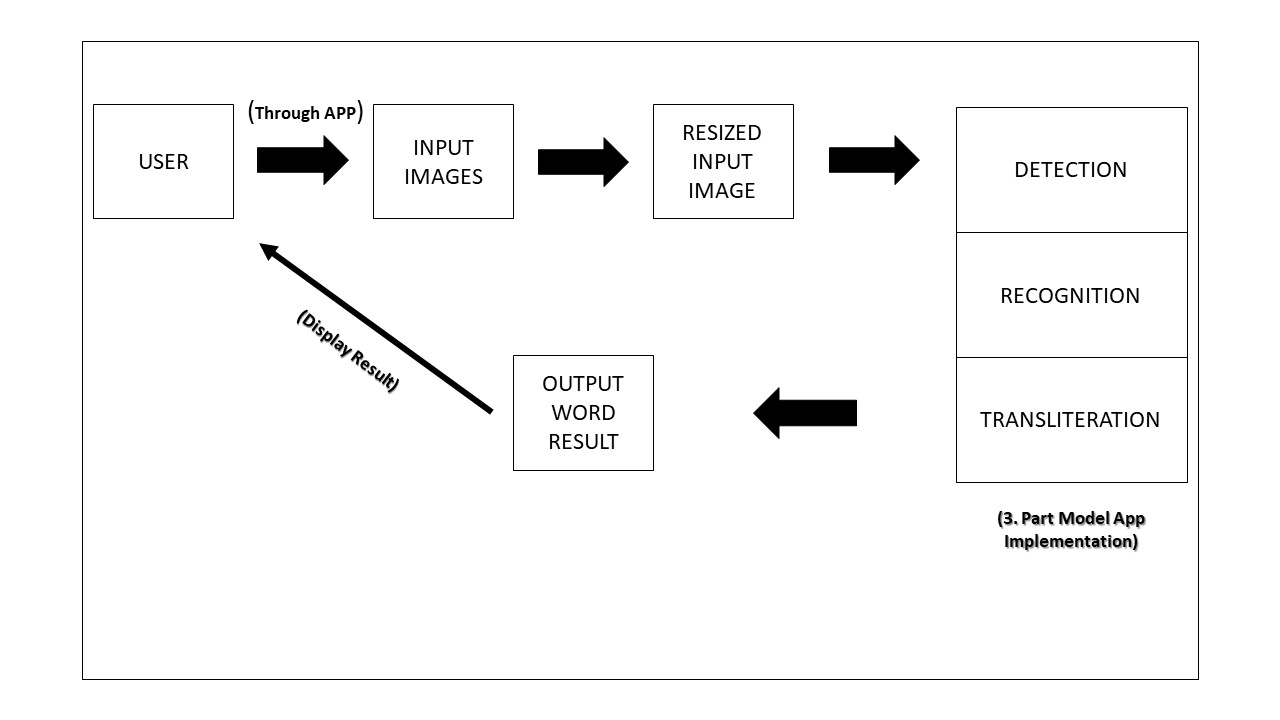
\includegraphics[scale=.3]{Slide2}}
				\caption{Functioning of App}
				\label{Slide2}
		\end{figure}
		\item The artificial neural network (ANN) behind the core functioning of the app is made up of 3 models performing consecutive tasks. That is, the output of a preceding model will be fed as input to the succeeding model, and thus they act as one model unit.
		\begin{figure}
				{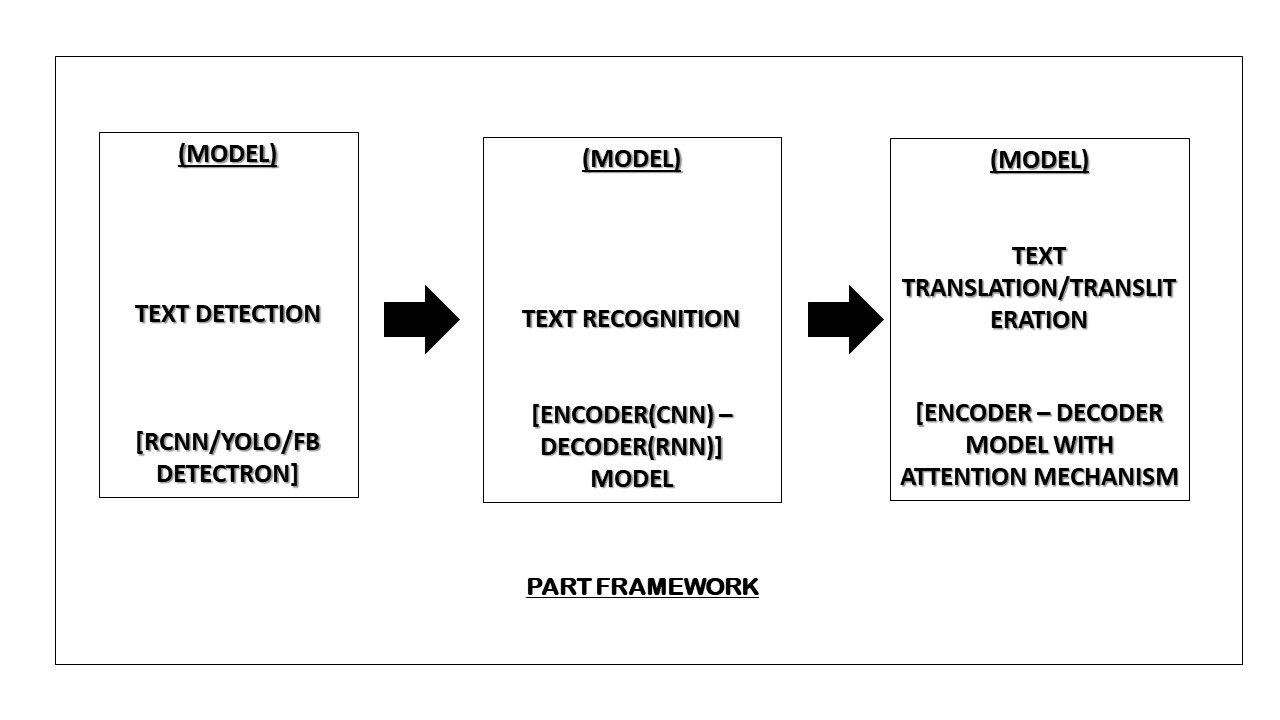
\includegraphics[scale=.3]{Slide1}}
				\caption{3-part model}
				\label{Slide1}
		\end{figure}
	\end{itemize}
\end{frame}


\section{Algorithms / Techniques to be used}
	\begin{frame}[allowframebreaks]{Techniques to be used}
	\begin{itemize}
		\item The 3 ANN models will be trained and tested on separate datasets curated to the task. The code for all the models will be written in Python using libraries such as PyTorch and Tensorflow, on Google Colab / Jupyter (.ipynb) notebooks, and using MLFlow for hyperparameter tuning. The models individually will perform the following tasks:
		\begin{itemize}
			\item The first task is \textbf{Text Detection}, a subset of object detection, and will performed by a Region-based Convolutional Neural Network (R-CNN). A classic R-CNN uses Support Vector Machines(SVMs) in its object-classifying stage, but for more efficient training and prediction, these will be replaced by a feedforward network. The possibility of using a You Only Look Once (YOLO) model will be explored.
			\item The second task is \textbf{Text Recognition}, which is a sequence labelling task. This will achieved by an Encoder- Decoder model. The encoder model will be a Convolutional Neural Network (CNN) which encodes input pciture of text into series of feature representations, while the decoder will be a Recurrent Neural Network (RNN) which extract text characters from the feature representations of the image. Connectionist Temporal Classification (CTC) loss will be used
			\item The third task will be \textbf{Text Translation / Transliteration}, that is, converting script from source language to target language and is a sequence-to-sequence generation task, which will again be a modelled by an Encoder - Decoder model, this time with both encoder and decoder being RNNs. The encoder will convert the input to an intermediate form. The decoder will then generate output in target script from this intermediate form. Attention mechanism will be implemented into the model.
		\end{itemize}
		\item These models will be then be deployed as a single unit onto the mobile app, either in pruned and compressed form or using Tensorflow Lite / Mobile.
		\item The app itself will be for Android platforms, and will be developed in Java.
	\end{itemize}
\end{frame}

\section{References}
\begin{frame}[allowframebreaks]{References}
	\bibliographystyle {abbrv}
	\bibliography {cite}
\end{frame}

\begin{frame}
	\begin{center}
	\LARGE
	\textcolor{red}{Thank You}
	\end{center}
\end{frame}
	

\end{document}